\documentclass[14pt]{extarticle}
\usepackage[english,ukrainian]{babel}
\usepackage[utf8]{inputenc}
\usepackage{amsmath,amssymb}
\usepackage{parskip}
\usepackage{graphicx}
\usepackage{xcolor}
\usepackage{tcolorbox}
\tcbuselibrary{skins}
\usepackage[framemethod=tikz]{mdframed}
\usepackage{chngcntr}
\usepackage{enumitem}
\usepackage{hyperref}
\usepackage{float}
\usepackage{subfig}
\usepackage{esint}
\usepackage[top=2.5cm, left=3cm, right=3cm, bottom=4.0cm]{geometry}
\usepackage[table]{xcolor}
\usepackage{algorithm}
\usepackage{algpseudocode}
\usepackage{listings}

\title{Контрольна робота з курсу ``Теоретична механіка''}
\author{Студента 3 курсу групи МП-31 Захарова Дмитра}
\date{\today}

\begin{document}

\maketitle

\begin{center}
\textbf{Варіант 3}
\end{center}

\section*{Завдання 1} 

\textbf{Умова.} Точкове тіло маси $m=10\,\text{кг}$ рухається зі стану спокою по колу з радіусом $R=20\,\text{м}$, розташованому в горизонтальній площині. Визначте шлях,
пройдений тілом за час $\tau = 5\,\text{с}$ після початку руху, якщо на тіло діє
горизонтальна сила $F = 20\,\text{Н}$, яка утворює сталий кут $\alpha=\frac{\pi}{4}$ з вектором швидкості. Тертям нехтуємо.

\textbf{Розв'язок.} 

Схематичний малюнок задачі зображено на рис.\ref{fig:1}.

\begin{figure}[H]
    \centering
    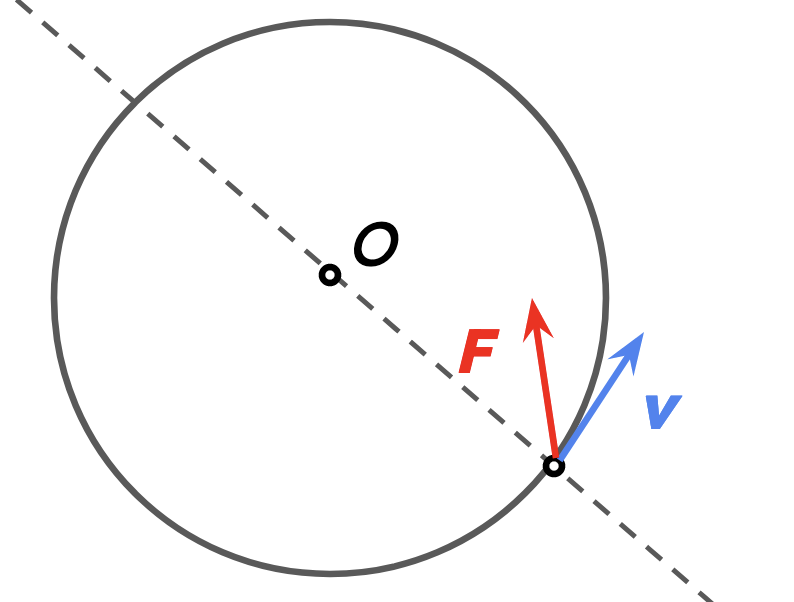
\includegraphics[width=0.4\textwidth]{images/test_2/problem_1.png}
    \caption{Ілюстрація до задачі 1}
    \label{fig:1}
\end{figure}

Запишемо проекцію на тангсенсальний напрямок:
\[
ma_{\tau} = F \cos\alpha \implies a_{\tau} = \frac{F \cos \alpha}{m}
\]
Тангенсальне прискорення $a_{\tau}=\frac{dv}{dt}=\text{const}$. Отже, швидкість від часу має вигляд $v(t)=\frac{Ft \cos\alpha}{m}$, а отже кутова швидкість $\omega(t) = \frac{Ft \cos\alpha}{mR}$. 

За час $\tau=5\,\text{с}$ зміна кута $\Delta \theta = \int_0^{\tau}\omega(t)dt$, а тоді шлях $s=R\Delta\theta$. Поєднуючи все, маємо:
\[
s = R\int_0^{\tau}\omega(t)dt = R \cdot \frac{F\tau^2 \cos\alpha}{2mR} = \frac{F\tau^2}{2\sqrt{2}m}
\]
Підставивши числа, маємо $s=\frac{25}{\sqrt{2}}\, \text{м}$. 

\textbf{Відповідь.} $s=\frac{F\tau^2}{2\sqrt{2}m}=\frac{25}{\sqrt{2}}\,\text{м}$.

\pagebreak
\section*{Завдання 2}

\textbf{Умова.} Яку мінімальну початкову кутову швидкість $\omega_0$ слід надати однорідному стержню довжиною $\ell=1\,\text{м}$, щоб він зміг здійснити
повний оберт навколо нерухомої горизонтальної осі $O$? Якою буде максимальна реакція осі?

\textbf{Розв'язок.} Під час руху, стрижень має деяку потенціальну та кінетичну енергію. Кінетична енергія скаладється лише з оберательної компоненти, причому момент інерції $I=\frac{1}{3}m\ell^2$. 

Розглянемо момент, коли стрижень повернувся на кут $\gamma$ від початкового положення. Тоді, якщо задати нульовий рівень за точку $O$, то на початку центр мас знаходиться на висоті $-\frac{\ell}{2}$, а потім $-\frac{\ell}{2}\cos \gamma$.

Тепер запишемо закон збереження енергії. Сума потенціальної і кінетичної енергії не змінюється: $T+V=\text{const}$.

На початку ця сума дорівнює:
\[
T_0 + V_0 = -mg\frac{\ell}{2}+\frac{I\omega_0^2}{2} = -mg\frac{\ell}{2} + \frac{m\ell^2\omega_0^2}{6}
\]
При куті $\gamma$:
\[
T(\gamma)+V(\gamma) = -mg \frac{\ell \cos\gamma}{2} + \frac{m\ell^2\omega^2}{6}
\]
Отже, в такому разі виконується
\[
-mg\frac{\ell}{2} + \frac{m\ell^2\omega_0^2}{6} = -mg\frac{\ell \cos\gamma}{2} + \frac{m\ell^2\omega^2}{6}
\]
Звідси дістаємо:
\[
\frac{m\ell^2(\omega_0^2-\omega^2)}{6} = \frac{mg\ell}{2}(1-\cos\gamma) \implies \omega_0^2-\omega^2 = \frac{3g}{\ell}(1-\cos\gamma)
\]
Якщо врахувати, що $1-\cos\gamma=2\sin^2{\frac{\gamma}{2}}$, то остаточно:
\[
\omega^2 = \omega_0^2 - \frac{6g}{\ell} \sin^2 \frac{\gamma}{2}
\]
Нас цікавить випадок, коли $\gamma=\pi$. В такому випадку швидкість буде $\omega^2 = \omega_0^2 - \frac{6g}{\ell}$. Щоб знайти саме мінімальне значення, помічаємо, що при крайньому випадку стрижень буде проходити верхнє положення з нульовою швидкістю. Тому, остаточно
\[
\boxed{\omega_{\min} = \sqrt{\frac{6g}{\ell}}}
\]
Знайдемо силу реакції опори $N$. Вважатимемо, що вона направлена уздовж стрижня. В такому разі, другий закон Ньютона в проекції на стрижень має вигляд:
\[
m\omega^2 \ell + mg \cos\gamma = N
\]
Враховуючи, що $\omega^2\ell=\omega_0^2\ell - 3g(1-\cos\gamma)$, маємо
\[
m\omega_0^2\ell - 3mg(1-\cos\gamma) + mg\cos\gamma = N
\]
Або, остаточно,
\[
N(\gamma) = m\omega_0^2\ell + mg(4\cos\gamma - 3)
\]
Екстремум досягається при або $\gamma=0$, або $\gamma=\pi$. Якщо підставляти наше конкретне $\omega_0=\omega_{\min}$, то
\[
N(\gamma) = 6mg + mg(4\cos\gamma - 3) = mg(3 + 4\cos\gamma)
\]
Бачимо, що максимум досягається при $\gamma=0$ і тоді $N_{\max}=7mg$. 

\textbf{Відповідь.} $\omega_{\min}=\sqrt{\frac{6g}{\ell}}, \; N_{\max}=7mg$.

\pagebreak
\section*{Завдання 3}

\textbf{Умова.} Гнучка нитка намотана на однорідний циліндр маси $m$ і радіуса $r$. Циліндр під дією сили тяжіння починає рухатися на похилій площині без початкової швидкості, долаючи тертя і розмотуючи нитку. Коефіцієнт тертя
дорівнює $\mu$. Визначте натяг $T$ нитки. Кут $\alpha$ вважаємо відомим.

\textbf{Розв'язок.} Розглянемо усі сили, що діють на циліндр: це сила натягу нитки $T$, сила нормальної реакції опори $N$, сила тяжіння $mg$ та сила тертя $F_f=\mu N$ (див. рис. \ref{fig:2})

\begin{figure}[H]
    \centering
    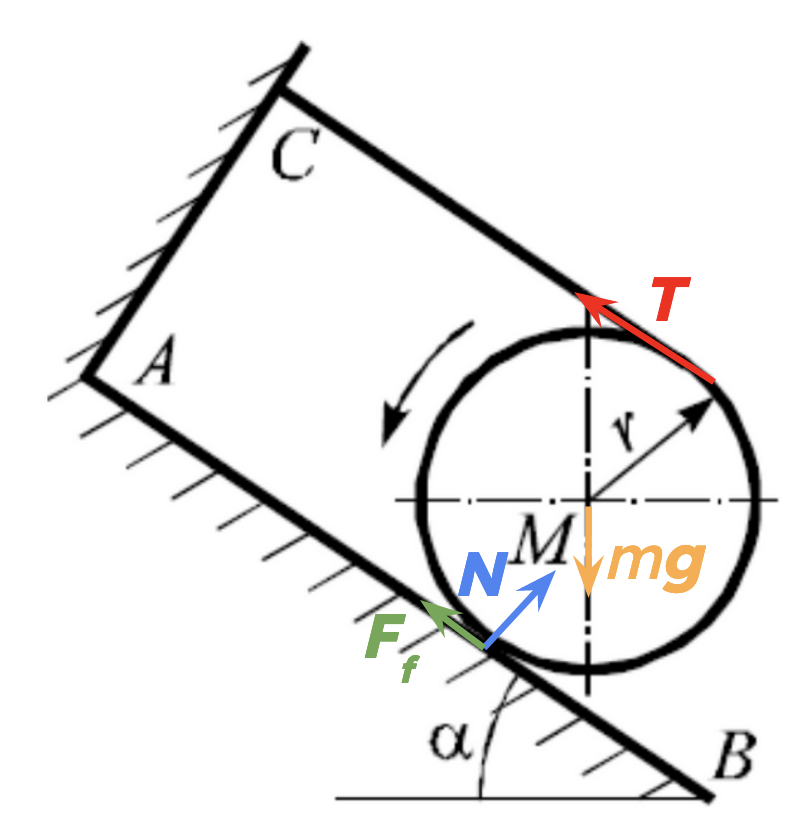
\includegraphics[width=0.5\textwidth]{images/test_2/problem_3.png}
    \caption{Сили, що діють на циліндр}
    \label{fig:2}
\end{figure}

Спроєктуємо другий закон Ньютона на вісь $Ox$ вздовж площини і перпендикулярно їй $Oy$:
\begin{gather*}
ma_x = -\mu N + mg \sin\alpha - T \\ 
ma_y = N - mg\cos\alpha 
\end{gather*}
Оскільки циліндр не рухається вздовж $Oy$, то $a_y=0$, а тому $N=mg\cos\alpha$. Підставляючи у друге:
\[
ma_x = -\mu mg \cos\alpha + mg\sin\alpha - T
\]
З іншого боку, ми можемо записати закон динаміки обертального руху:
\[
I\varepsilon = Tr - \mu N r
\]
Момент інерції суцільного циліндру $I = \frac{mr^2}{2}$. В такому разі:
\[
\frac{mr^2\varepsilon}{2} = Tr - \mu mgr \cos\alpha \implies \varepsilon = \frac{2T}{mr} - \frac{2\mu g \cos\alpha }{r}
\]
Кутове прискорення пов'язане з прискоренням співвідношенням $\varepsilon = \frac{a_x}{r}$. Таким чином
\[
a_x = \frac{2T}{m} - 2\mu g \cos\alpha
\]
Отже, підставляючи у другий закон Ньютона:
\begin{gather*}
2T - 2\mu mg \cos\alpha = -\mu mg \cos\alpha + mg \sin \alpha - T \\
3T = \mu mg \cos\alpha + mg\sin \alpha \\
\boxed{T = \frac{mg}{3}(\mu \cos\alpha + \sin \alpha)}
\end{gather*}

\textbf{Відповідь.} $T=\frac{\mu \cos\alpha+\sin\alpha}{3}\cdot mg$.

\end{document}

